\section{Problem and Motivations}

Modern distributed file systems, such as GFS\cite{ghemawat2003google}, HDFS\cite{shvachko2010hadoop}, Ceph\cite{weil2006ceph}, which consist of three components, metadata servers(MDS), object-based storage devices(OSD) and clients as Fig.~\ref{fig:architecture} shows. Clients perform metadata operations(\emph{open, stat}) directly with MDS and file I/O directly with data server. This architecture decouples metadata I/O from data IO and increases overall scalability. For example, client requests data with pathname /var/log/client.log. By multiple interactions to MDS, client lookups the directory of \texttt{root}, \texttt{var} and \texttt{log} to locate the inode of \texttt{client.log} and checks the permission. Once client obtain the inode, it must get the capability to access to data. Then, client will request a lease on this file to MDS. Finnaly, client interact with OSD to operator file I/O. Due to the iterative lookup and checking permission operations, the IOs between clients and MDS are more than OSD. Because overall 50\% of IOs are to metadata\cite{roselli2000comparison}, metadata performance is crucial.

Especially in web content system, loading one web file leads to multiple scripts and images requesting. We analyse the access log\cite{zhang2016composite} of web server and find that there are 23\% of requests are correlated. These too frequently correlated metadata fetching increases the traffic to MDS and network. If there is no optimization on metadata fetching, too more traffic will overwhelm MDS and becomes a bottleneck in the system.

\begin{figure}[htbp]
  \centering
  % Requires \usepackage{graphicx}
  %\vspace{-5pt}
  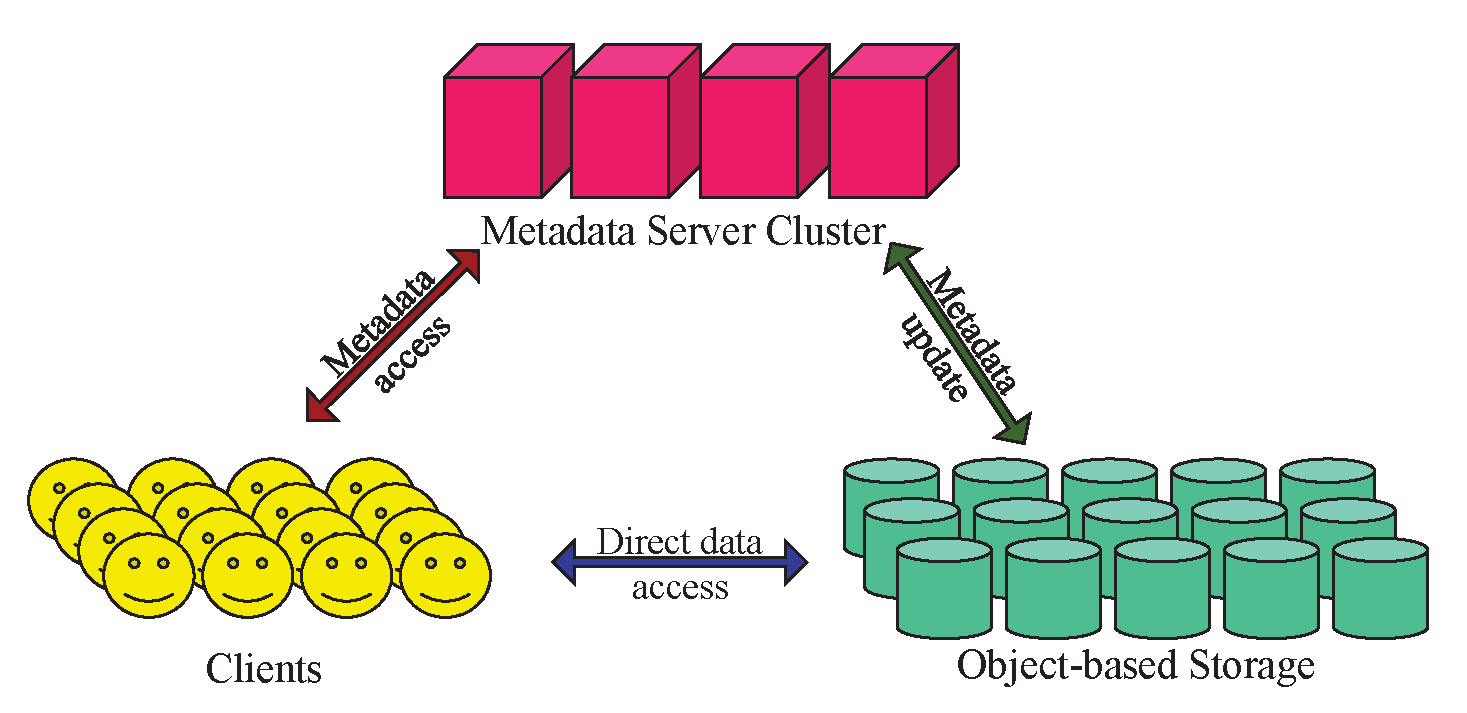
\includegraphics[width=1\linewidth]{architecture.eps}\\
  %\vspace{-10pt}
  \caption{Architecture of distributed file systems.}\label{fig:architecture}
   %\vspace{-10pt}
\end{figure}

In this paper, we propose a correlations-based metadata prefetching to reduce IO traffic to MDS, to scale distributed file systems, to increase client cache hit ratio with high accuracy and low false positive. How to define the correlations among files and how to update correlations in real time become a challenge.
